%% Section 4: RevTrace system.

RevTrace realizes DGFT with family adapters, a two-plane coordinator, a
versioned ledger, and contract-scoped certification (Fig.~\ref{fig:arch}).

\begin{figure*}[t]
  \centering
  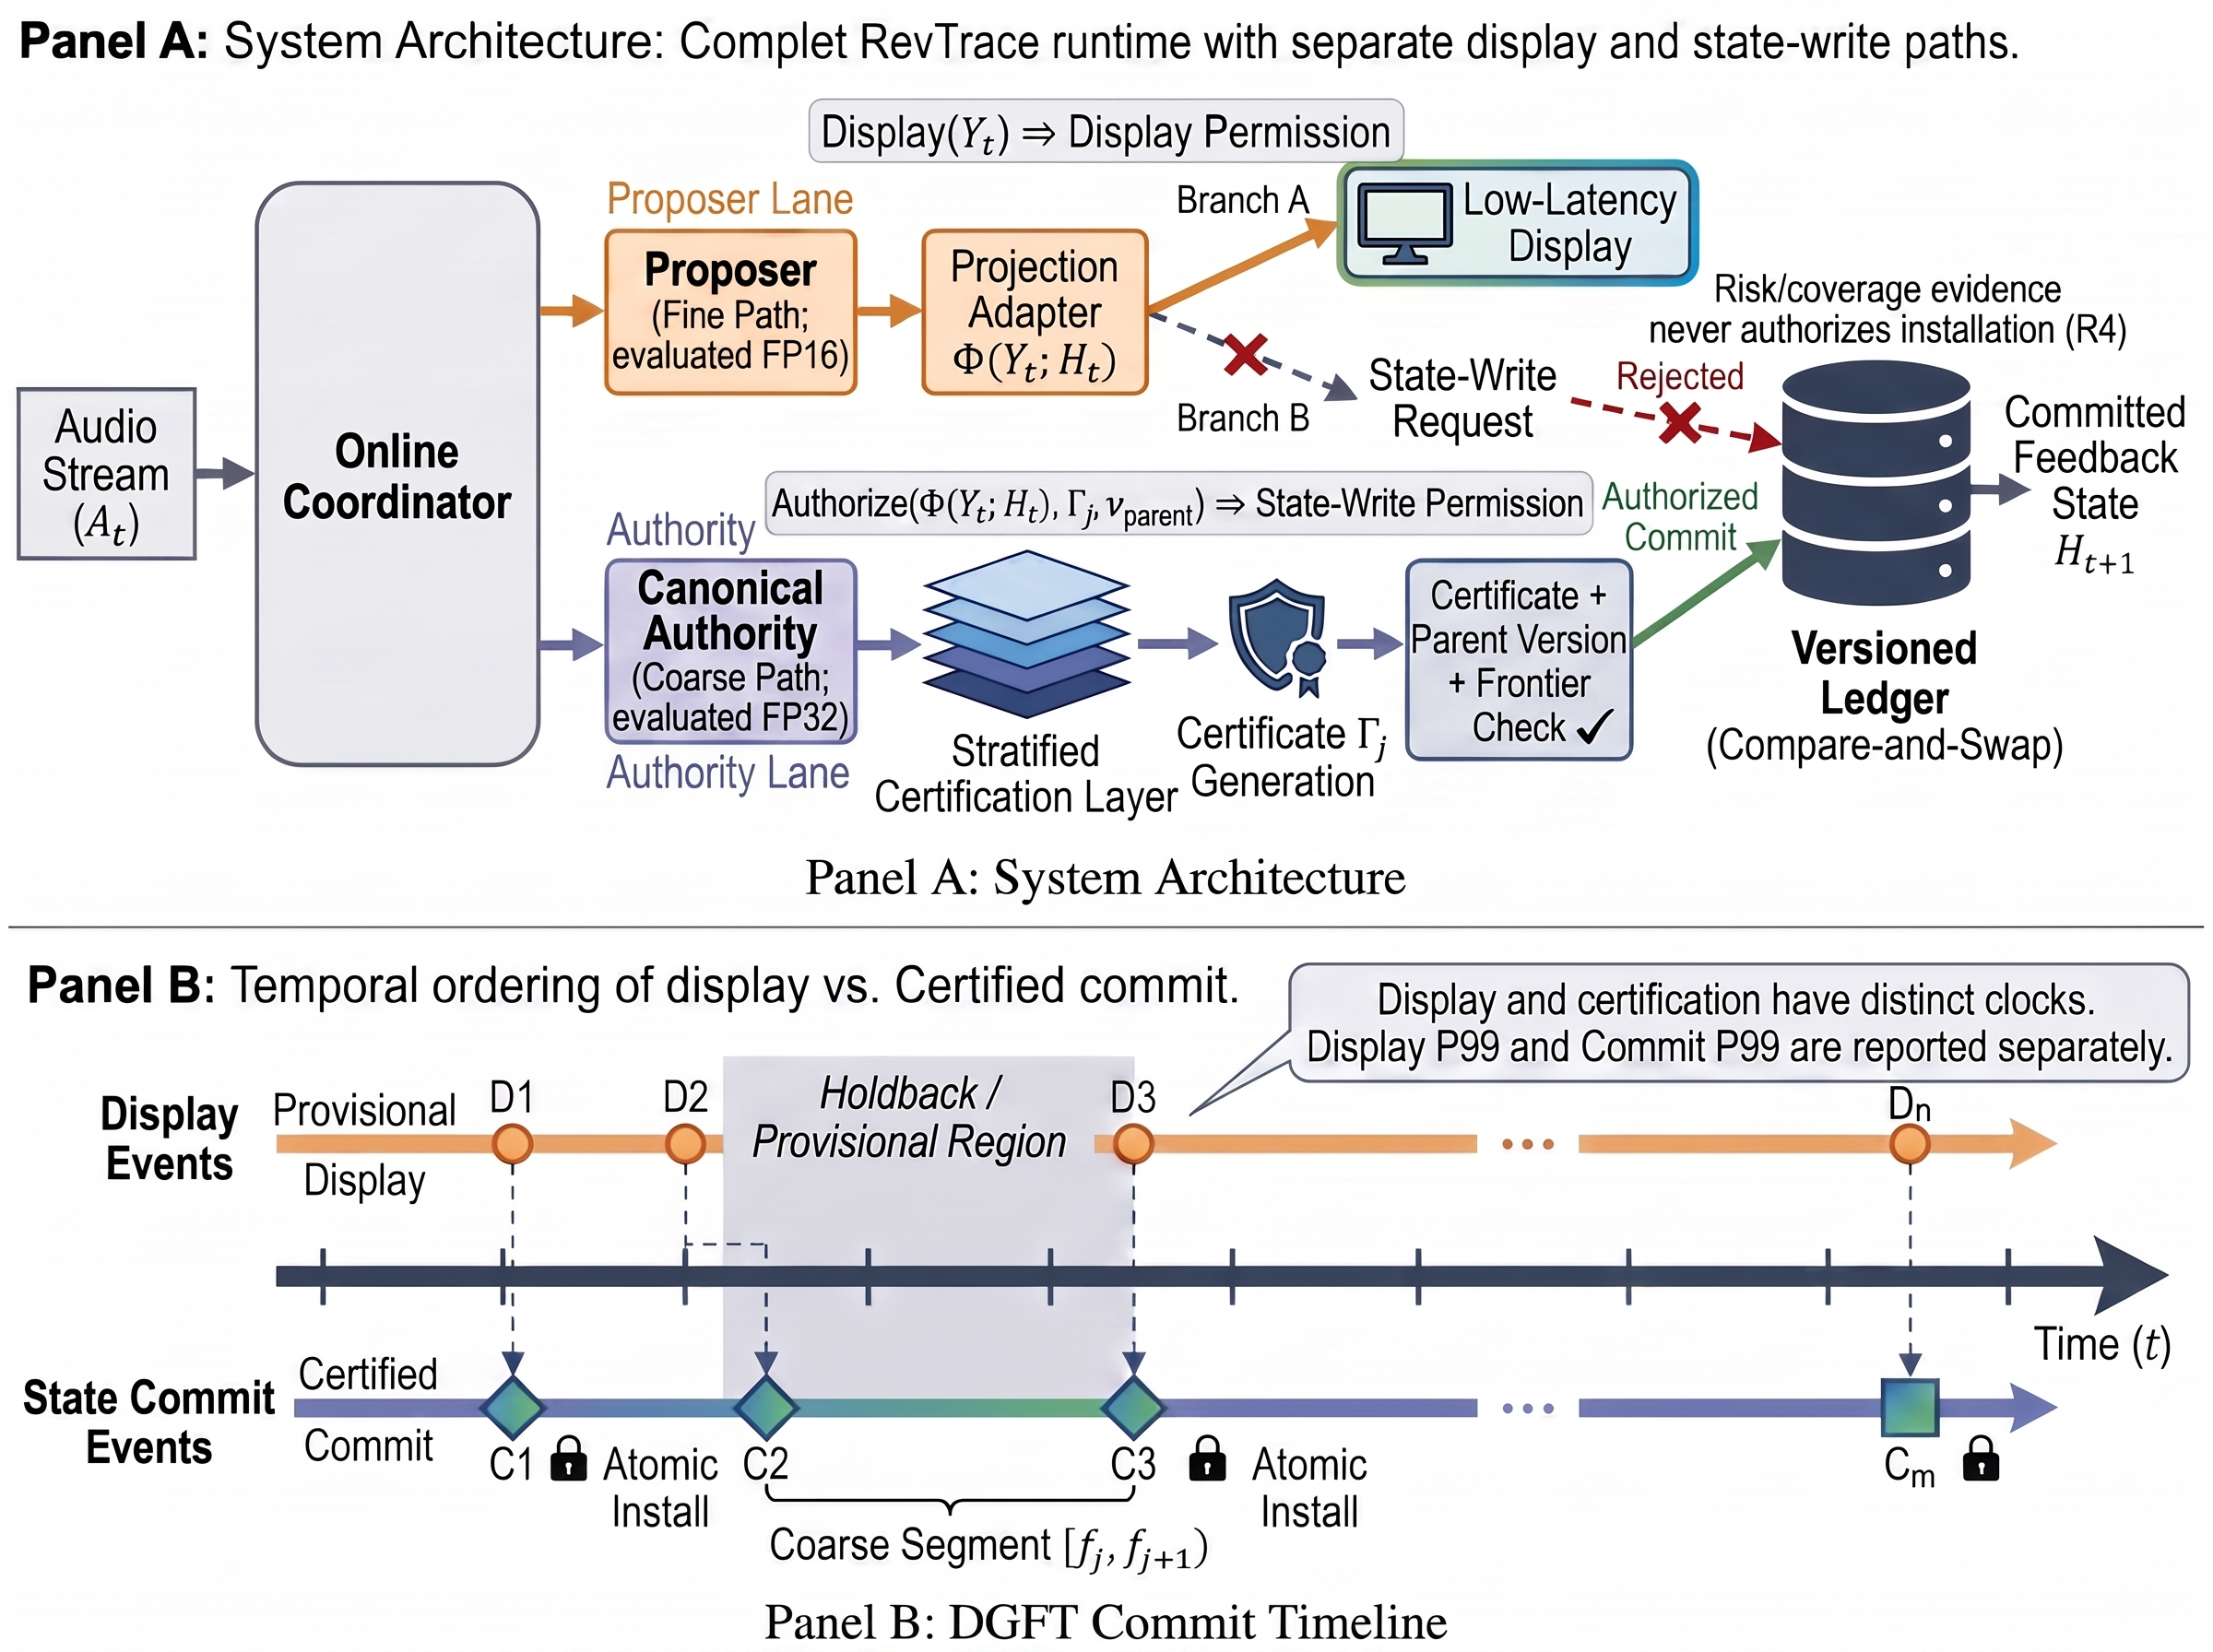
\includegraphics[width=0.94\textwidth]{figures/f2_architecture_senior.jpg}
  \caption{RevTrace architecture and commit timeline. Proposal may drive
  low-latency display, but only a certificate bound to the current parent and
  frontier may install state. FP32 is the evaluated coarse authority, not a
  protocol requirement.}
  \label{fig:arch}
\end{figure*}

\subsection{Adapters and two-plane coordination}\label{sec:sys:adapters}

Each model family supplies three interfaces: a projection adapter computing
$\proj(\out_t;H_t)$ (Qwen rollback prefix or Whisper previous-text prompt), an
authority adapter executing its canonical path, and an evidence adapter that
collects margins, directional coverage, and repetition signals. The online
coordinator runs proposer and authority on separate GPUs, invalidates stale
descendants (Corollary~\ref{cor:stale}), closes terminal frontiers, and rebases
displayed provisional state after superseding commits. RQ3 evaluates the same
runtime through both family adapters. A slow authority may delay certified
commit without blocking provisional display; the evaluation consequently
reports display and commit clocks separately.\label{sec:sys:coord}

\subsection{Certificate ledger}\label{sec:sys:ledger}

The compare-and-swap ledger stores the committed version and audio frontier.
Before installation it matches each $\commit_j$ against the session, contract
epoch, policy, parent-version, frontier, and certificate-consumption fences.
RQ2 exhaustively records these checks for every install attempt.

\subsection{Coverage and selective replay}\label{sec:sys:coverage}

A coarse certificate records, in Latin or CJK units, which proposal regions it
covers. Uncovered regions enter fine replay; Hybrid additionally replays
risk-selected regions at fraction $r$. Coverage therefore controls work but
does not grant write authority. RQ3 compares Coarse ($r=0$) and Hybrid ($r>0$)
under a matched workload.

\subsection{Stratified certification}\label{sec:sys:cert}

The four non-transferable strata in Fig.~\ref{fig:cert} are: (i) randomized,
anytime-valid UCB audits of SG numerical risk, scoped only to the SG adapter
path~\cite{howard2021confidence,ramdas2023savi}; (ii) fail-closed,
contract-scoped preflight tests of authority repeatability and
batch-vs-singleton invariance; (iii) exhaustive online certificate, version,
and frontier validation; and (iv) independent family-specific semantic
references. Evidence may schedule verification but never authorize a state
write (R4). The separation prevents a favorable statistical bound in one
contract from being promoted into an installation certificate for another.

\begin{figure*}[t]
  \centering
  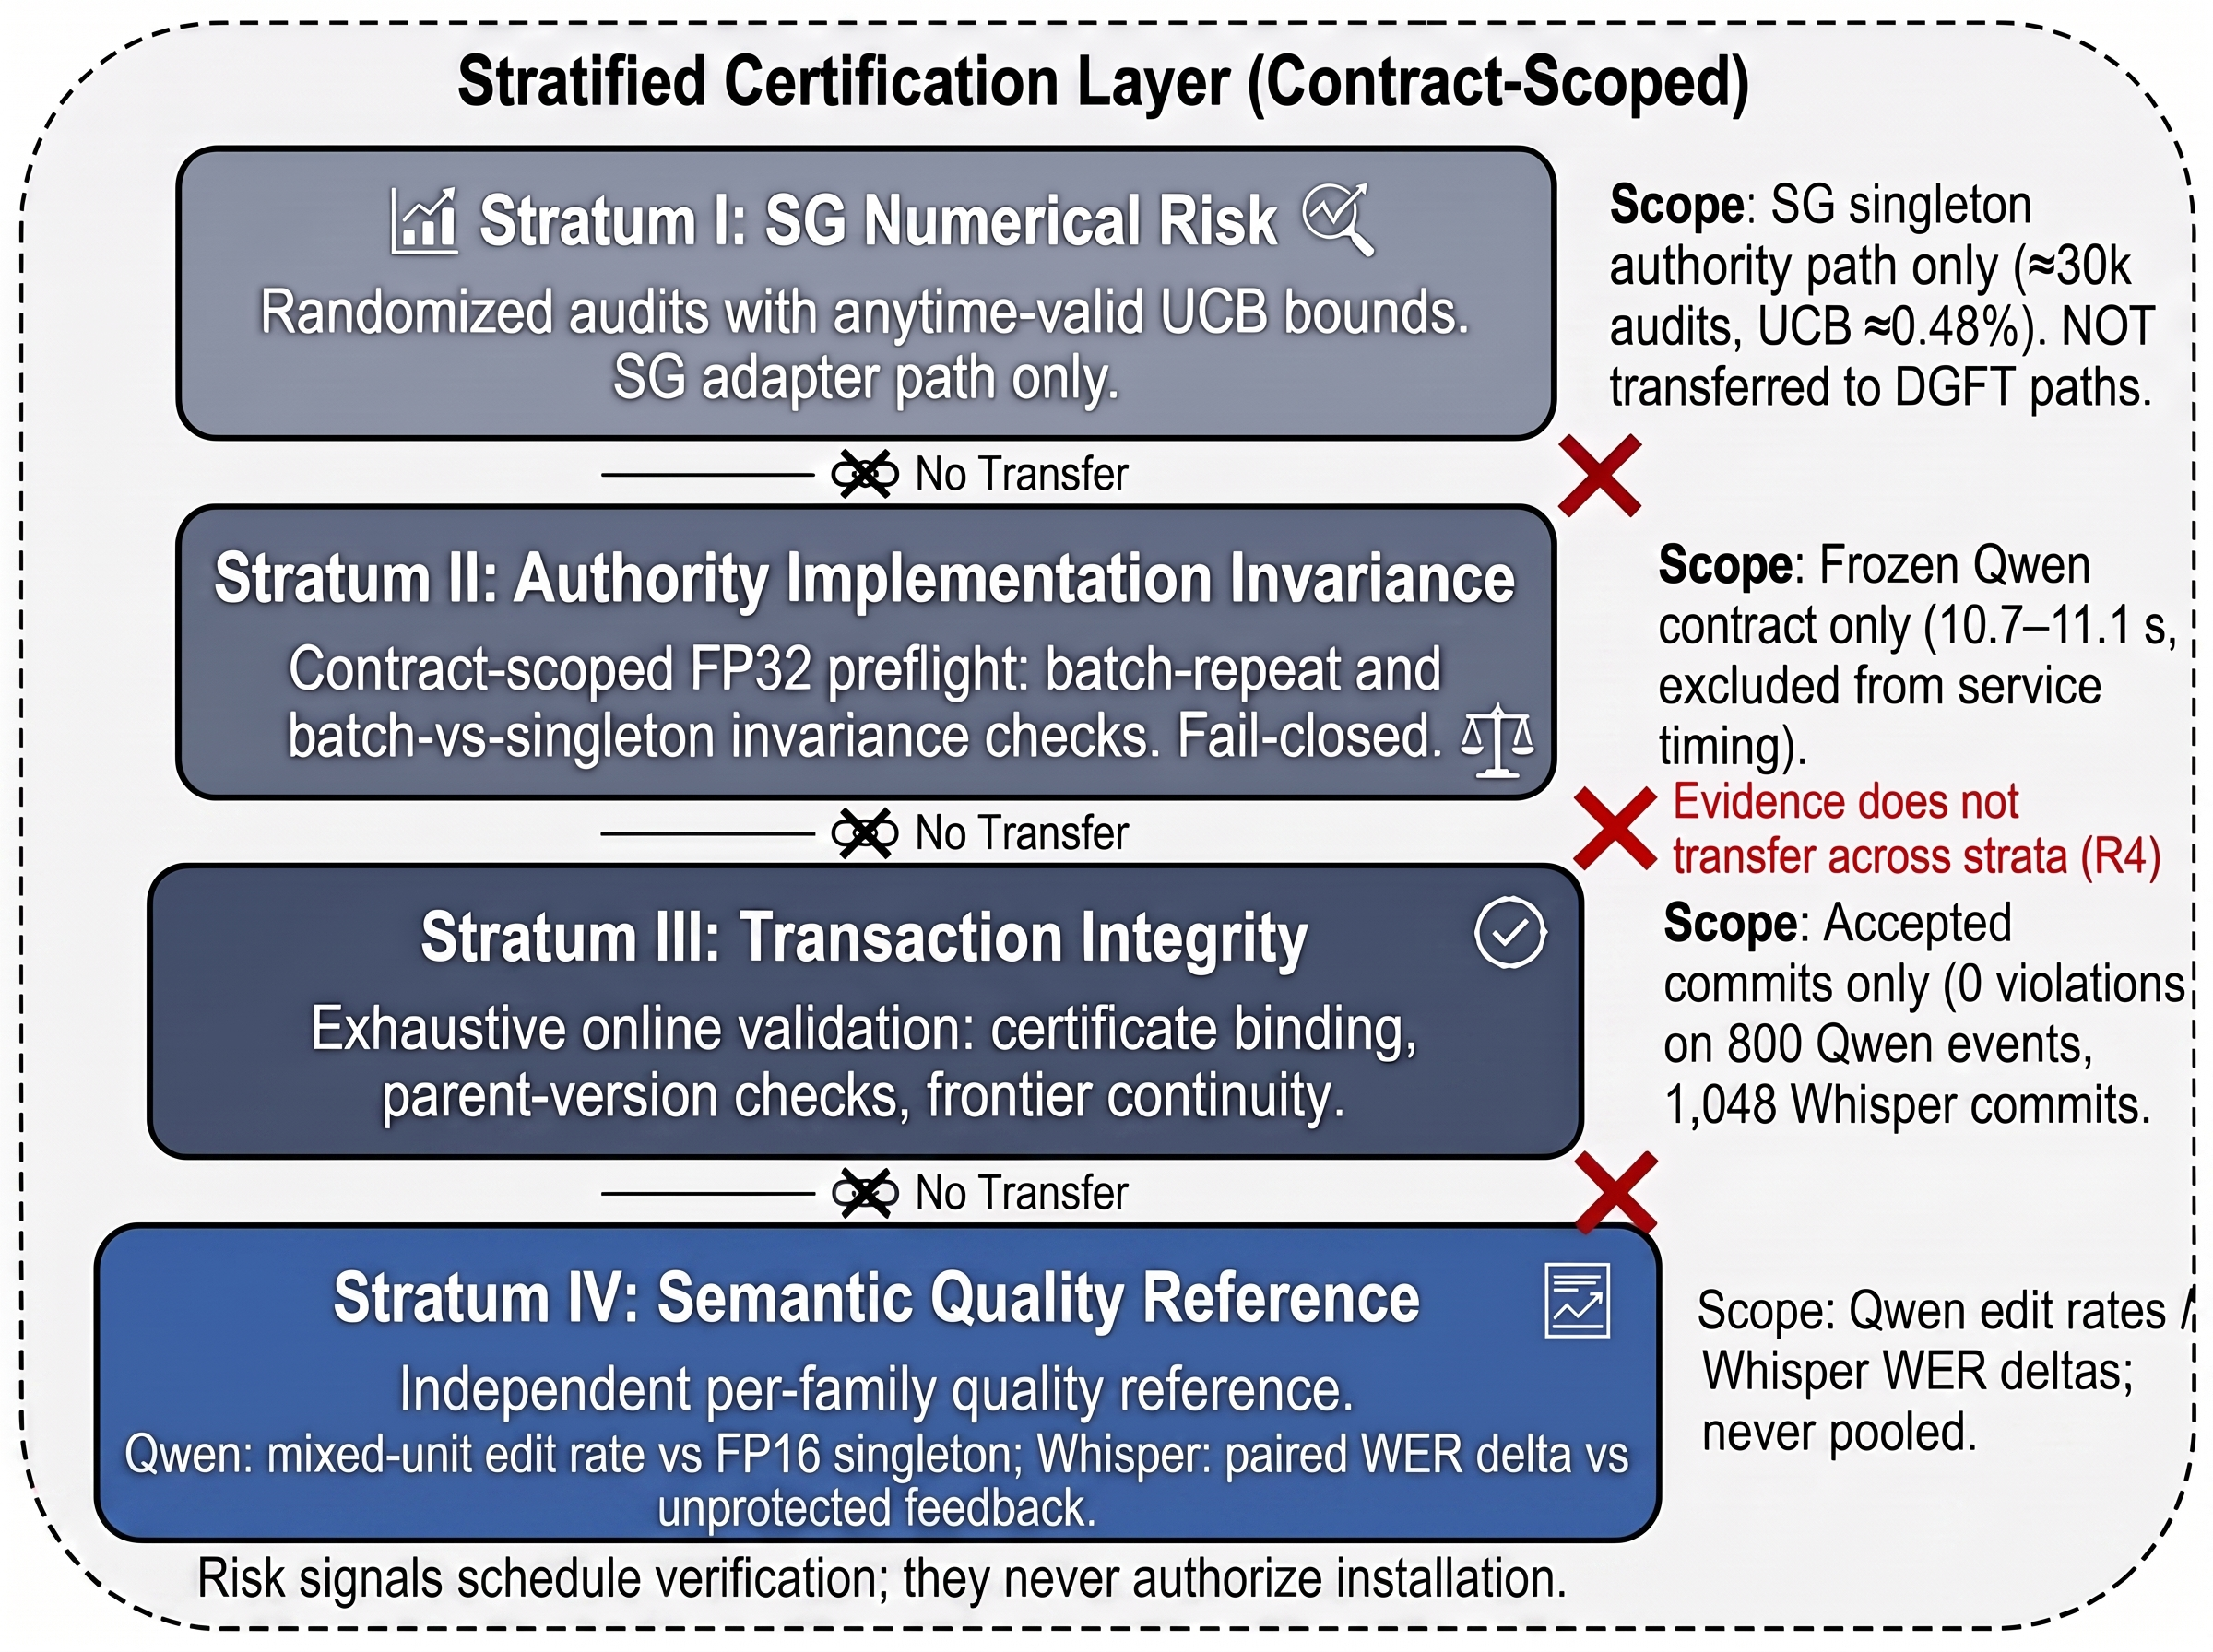
\includegraphics[width=0.92\textwidth]{figures/f3_certification_senior.jpg}
  \caption{Contract-scoped certification. Each stratum supports only its stated
  guarantee; evidence never transfers across strata. Qwen and Whisper quality
  estimands remain separate.}
  \label{fig:cert}
\end{figure*}
